% ============= setup ============= %
% ======== package ======== %
\documentclass[mathserif]{beamer}
\usepackage{xeCJK}
\usepackage{graphicx}
\usepackage{xcolor}
\usepackage{setspace}
\usepackage{newtxmath}
\usepackage{chemfig}

% ======== font ======== %
\setCJKmainfont{Taipei Sans TC Beta}
\setCJKsansfont{Taipei Sans TC Beta}
\AtBeginDocument{%
    \DeclareSymbolFont{pureletters}{OML}{cmm}{m}{it}%
    \SetSymbolFont{pureletters}{bold}{OML}{cmm}{b}{it}%
}
\hypersetup{
    colorlinks=true,
    linkcolor=black,
    urlcolor=blue
}

% ======== theme ======== %
\renewcommand{\baselinestretch}{1.25}
\usetheme{Madrid}
\usecolortheme{crane}
\setbeamertemplate{items}[circle]
\setbeamertemplate{section in toc}{\inserttocsectionnumber.~\inserttocsection}
\AtBeginSection[]{
    \begin{frame}
        \vfill
        \centering
        \begin{beamercolorbox}[sep=8pt,center,shadow=true,rounded=true]{title}
            \usebeamerfont{title}\insertsectionhead\par%
        \end{beamercolorbox}
        \vfill
    \end{frame}
}

% ======== data ======== %
\title{LaTeX}
\author{temmie}
\date{}

% ============= setup ============= %

\begin{document}

\begin{frame}
    \titlepage
\end{frame}

\begin{frame}
    \tableofcontents
\end{frame}

\section{LaTeX 簡介}

\begin{frame}
    \frametitle{簡介}
    \begin{itemize}
        \item 是一種\textbf{用文字製作檔案}的語言
        \item 可以快速解決排版、複雜表格、數學公式
        \item 在學術界非常常用,主要是用來製作論文
        \vspace{0.5cm}
        \item $LaTeX \neq latex$
    \end{itemize}
\end{frame}

\begin{frame}
    \frametitle{數學式演示}
    $$ax^2+bx+c=0$$

    $$x=\frac{-b\pm \sqrt{b^2-4ac}}{2a}$$
\end{frame}

\begin{frame}
    \frametitle{數學式演示}
    $$F(A) = V \cdot a = \begin{bmatrix}
    1 & x_0^1 & \cdots & x_0^{n-1} \\
    1 & x_1^2 & \cdots & x_1^{n-1} \\
    \vdots & \vdots & \vdots & \vdots \\
    1 & x_{n-1}^2 & \cdots & x_{n-1}^{n-1}
    \end{bmatrix}
    \begin{bmatrix}
    a_0 \\
    a_1 \\
    \vdots \\
    a_{n-1}
    \end{bmatrix}$$
\end{frame}

\begin{frame}
    \frametitle{數學式演示}
    \begin{equation}
        \label{eq:multivariable_integral}
        \iiint_V f(x,y,z),dV = \int_a^b \int_{\phi_1(x)}^{\phi_2(x)} \int_{\psi_1(x,y)}^{\psi_2(x,y)} f(x,y,z),dz,dy,dx
    \end{equation}
    \begin{center}
        (請不要在意這個公式是不是正確的)
    \end{center}
\end{frame}

\begin{frame}
    \frametitle{結構式演示}
    \begin{center}
        \chemfig{C(-[2]H)(-[4]H)(-[6]H)(-[0]H)}
        \vspace{0.5cm}

        $CH_4$
    \end{center}
\end{frame}

\begin{frame}
    \frametitle{結構式演示}
    \begin{center}
        \chemfig{*6((=O)-(-(=[:150]O)-[:210]*6(-=-(-CH_3)-=-))-=-(-CH_3)-=)}
    \end{center}
\end{frame}

\section{優點 & 使用經驗}

\begin{frame}
    \frametitle{優點}
    \begin{itemize}
        \item 不會跑版
        \item 支援多種套件
        \item 不用自己處理目錄或是頁碼
        \item 數學式很好看 uwu
    \end{itemize}
\end{frame}

\begin{frame}
    \frametitle{使用經驗}
    \begin{center}
        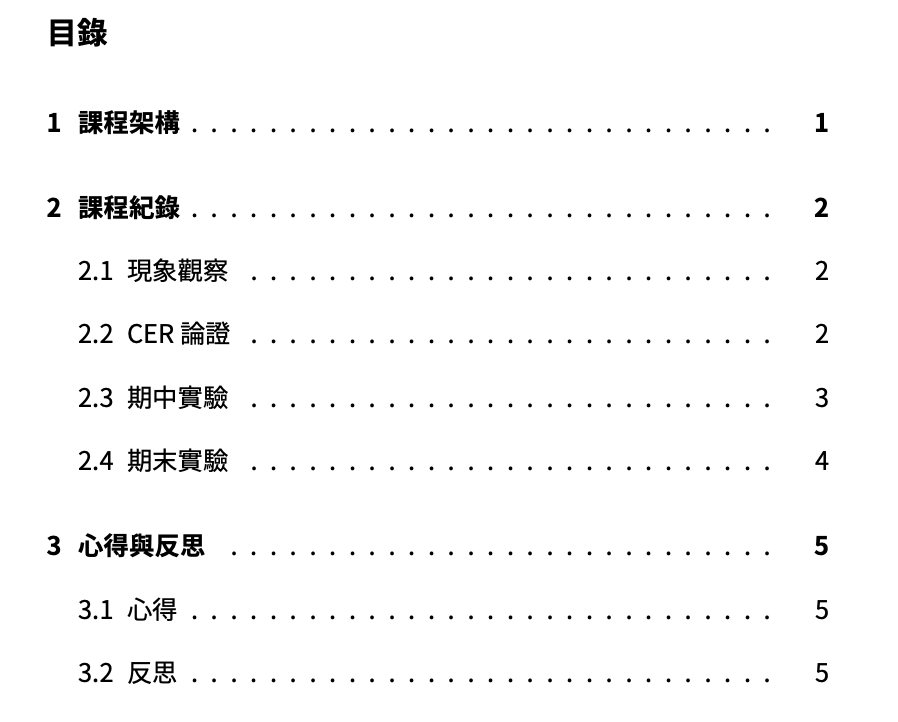
\includegraphics[width=7.0cm]{img/example1.png}
        
        $\blacktriangle$ 某次學習歷程的目錄
    \end{center}
\end{frame}

\begin{frame}
    \frametitle{使用經驗}
    \begin{center}
        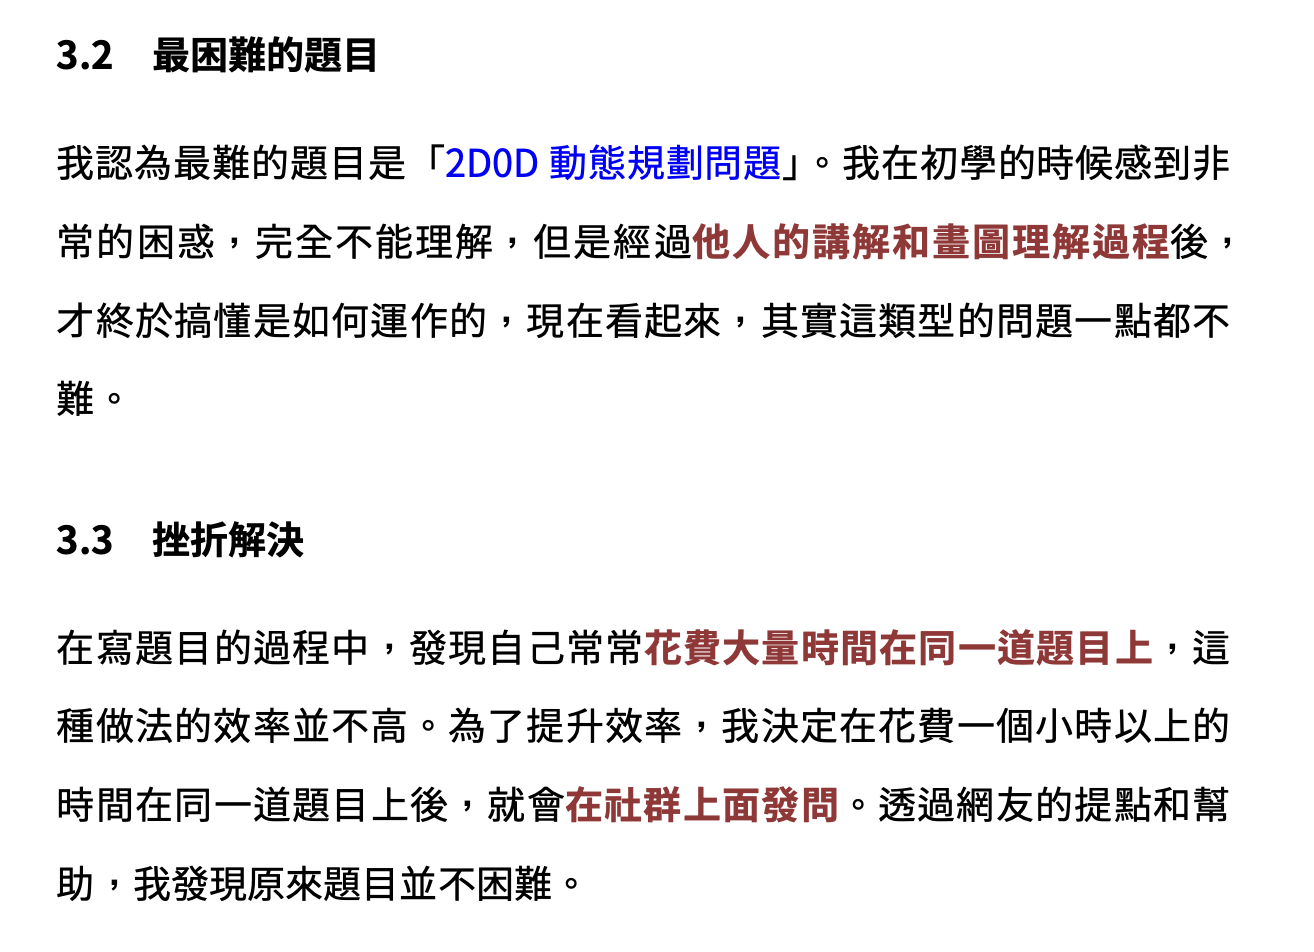
\includegraphics[width=8.0cm]{img/example2.png}
        
        $\blacktriangle$ 某次學習歷程的內容
    \end{center}
\end{frame}

\begin{frame}
    \frametitle{使用經驗}
    \begin{center}
        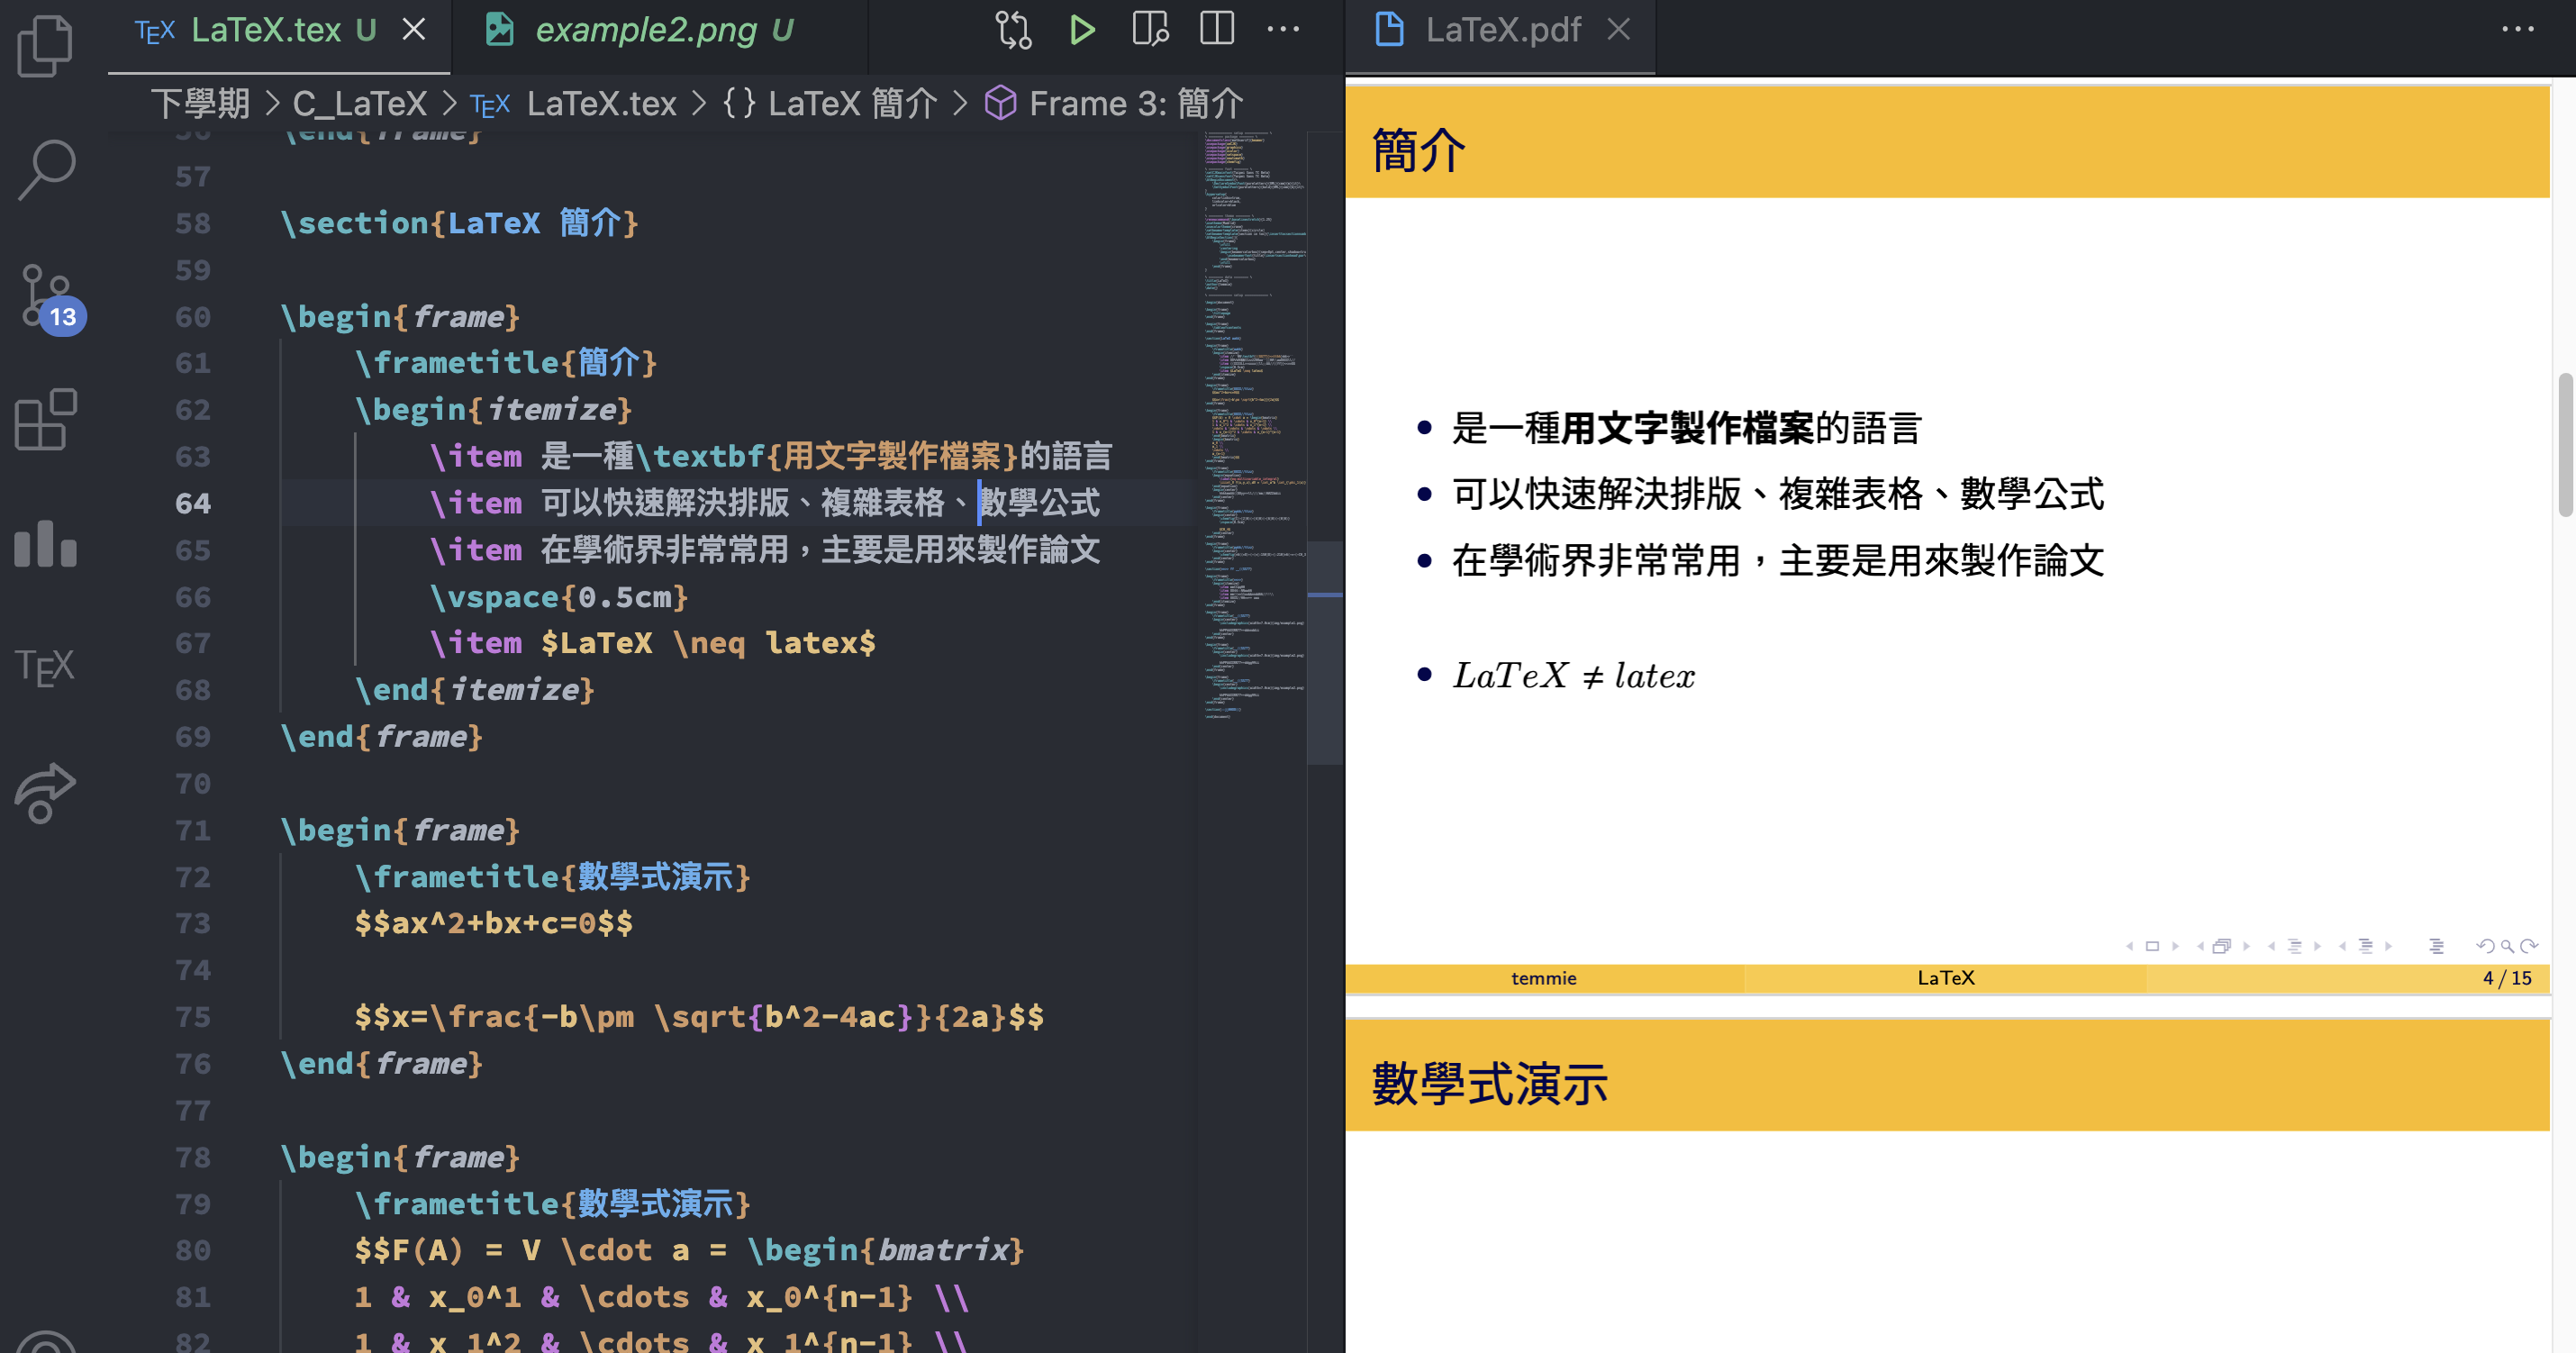
\includegraphics[width=10.0cm]{img/example3.png}
        
        $\blacktriangle$ 這份簡報
    \end{center}
\end{frame}

\section{線上編輯器}

\begin{frame}
    \frametitle{線上編輯器}
    \begin{itemize}
        \item 由於完整的 LaTeX 環境過大,我們今天會使用線上編輯器教學
        \item \href{https://www.overleaf.com}{Overleaf 網頁}
    \end{itemize}
\end{frame}

\begin{frame}
    \frametitle{編輯器畫面}
    \begin{center}
        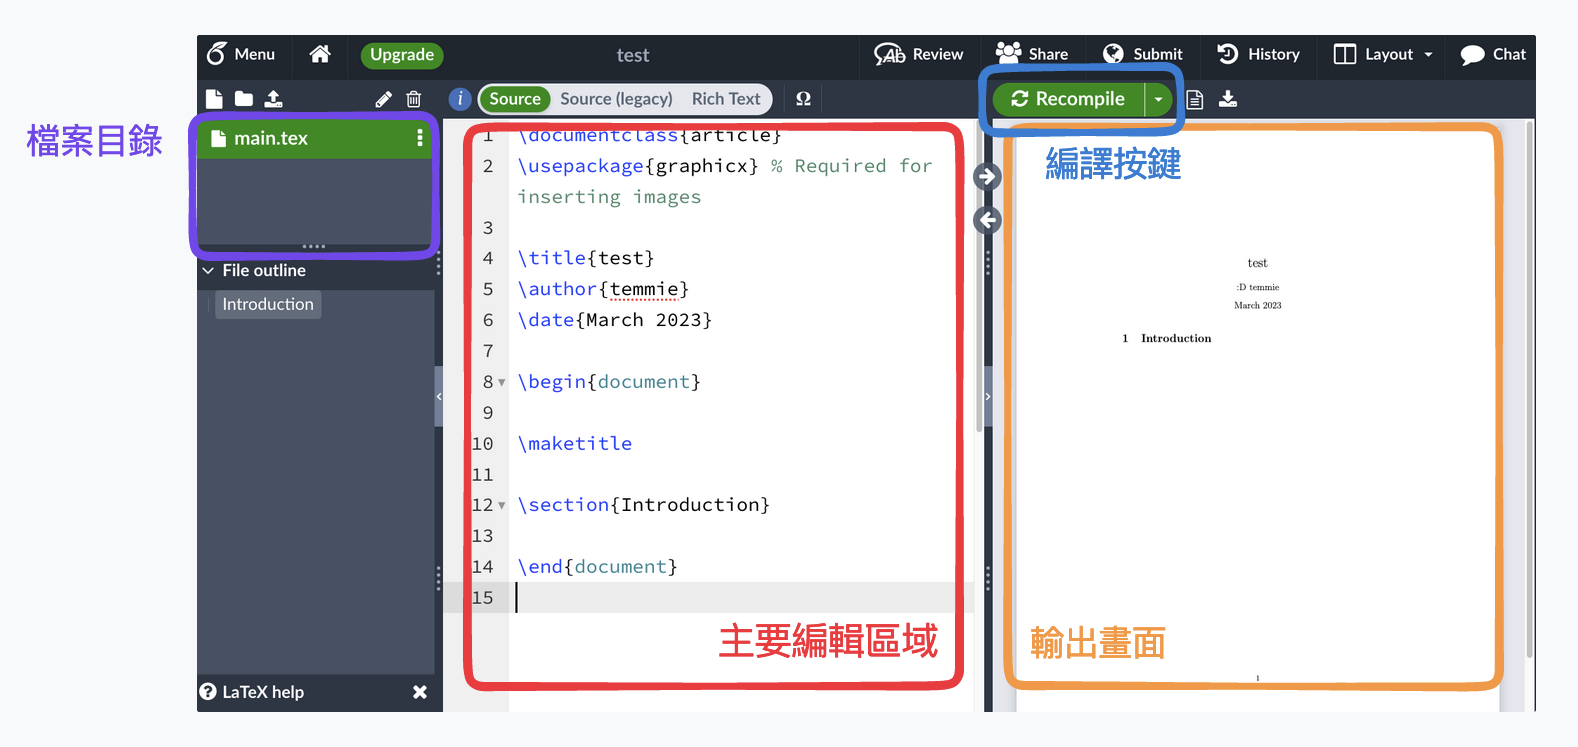
\includegraphics[width=12.0cm]{img/editor.png}
    \end{center}
\end{frame}

\begin{frame}
    \frametitle{設定}
    \begin{itemize}
        \item 由於之後會有中文的設定,請把 Compiler 設定成 XeLaTeX
        \item 左上 Menu → Setting → Compiler → XeLaTeX
    \end{itemize}
\end{frame}

\section{LaTeX 語法}

\begin{frame}
    \frametitle{基本模板}
    請參閱本講義目錄中 code/template.tex 檔案

\end{frame}

\begin{frame}
    \frametitle{章節設定}
    \begin{itemize}
        \item {\color{red}{\textbackslash section}} 設定大標題
        \item {\color{red}{\textbackslash subsection}} 設定子標題
        \vspace{0.5cm}
        \item 以上會同步到目錄上面
    \end{itemize}
\end{frame}

\begin{frame}
    \frametitle{頁面配置}
    \begin{itemize}
        \item 換行
            \begin{itemize}
                \item {\color{red}{\textbackslash\textbackslash}}
                \item 做兩次換行
            \end{itemize}
        \item 文字間距
            \begin{itemize}
                \item {\color{red}{\textbackslash vspace\{間距cm\}}}
            \end{itemize}
    \end{itemize}
\end{frame}

\begin{frame}
    \frametitle{文字效果}
    \begin{itemize}
        \item 粗體
            \begin{itemize}
                \item {\color{red}{\textbackslash textbf\{文字\}}}
            \end{itemize}
        \item 斜體
            \begin{itemize}
                \item {\color{red}{\textbackslash textit\{文字\}}}
            \end{itemize}
    \end{itemize}
\end{frame}

\begin{frame}
    \frametitle{圖片插入}
    \begin{itemize}
        \item 插入圖片
            \begin{itemize}
                \item {\color{red}{\textbackslash includegraphics[width=圖片長度]\{檔案名稱\}}}
            \end{itemize}
    \end{itemize}
\end{frame}

\begin{frame}
    \frametitle{列表}
    \begin{itemize}
        \item 列表
            \begin{itemize}
                \item {\color{red}{
                    
                \textbackslash begin\{列表類別\}\\
                \hspace{0.5cm} \textbackslash item 資訊\\
                \textbackslash end\{列表類別\}\\
                
                }}

            \end{itemize}
        \item 列表類別
            \begin{itemize}
                \item itemize:無序列表
                \item enumerate:有序列表
            \end{itemize}
    \end{itemize}
\end{frame}

\begin{frame}
    \frametitle{數學公式}
    \begin{itemize}
        \item 段落內公式框
            \begin{itemize}
                \item {\color{red}{\$你的公式\$}}
            \end{itemize}
        \item 獨立公式框
            \begin{itemize}
                \item {\color{red}{
                    
                \textbackslash [\\
                \hspace{0.5cm} 你的公式\\
                \textbackslash ]\\
                
                }}
            \end{itemize}
    \end{itemize}
\end{frame}

\begin{frame}
    \frametitle{數學公式}
    \begin{itemize}
        \item 上標
            \begin{itemize}
                \item 3x\^{}2+7x\^{}2+5
                \item $3x^2+7x^2+5$
            \end{itemize}
        \item 下標
            \begin{itemize}
                \item a\_{}i+a\_{}j>a\_{}k
                \item $a_i+a_j>a_k$
            \end{itemize}
        \item 分數
            \begin{itemize}
                \item \textbackslash frac\{1\}\{2\}
                \item $\frac{1}{2}$
            \end{itemize}
    \end{itemize}
\end{frame}

\section{參考資料}

\begin{frame}
    \frametitle{參考資料}   
    \begin{itemize}
        \item \href{https://youtu.be/mQamBS6uTOc}{教學影片}
        \item \href{https://hackmd.io/@CynthiaChuang/Basic-LaTeX-Commands}{數學符號指令}
    \end{itemize}
\end{frame}

\end{document}